
\chapter{生产者、生产者与市场效率}

福利经济学(welfare economics):研究自研配置如何影响经济福利的一门学问。


\section{消费者剩余}

\subsection{支付意愿}

每一个买者愿意支付的最高价格称为\keyword{支付意愿(willingness to pay)},
它衡量买者对物品的评价。


消费者剩余(consumer surplus)是买者愿意为一种物品支付的量减去其为此实际支付的量。
消费者剩余衡量买者从参与市场中得到的利益。

边际买者(marginal buyer)是指如果价格再提高一点就首先离开市场的买者。


\begin{figure}[!ht]
  \centering
  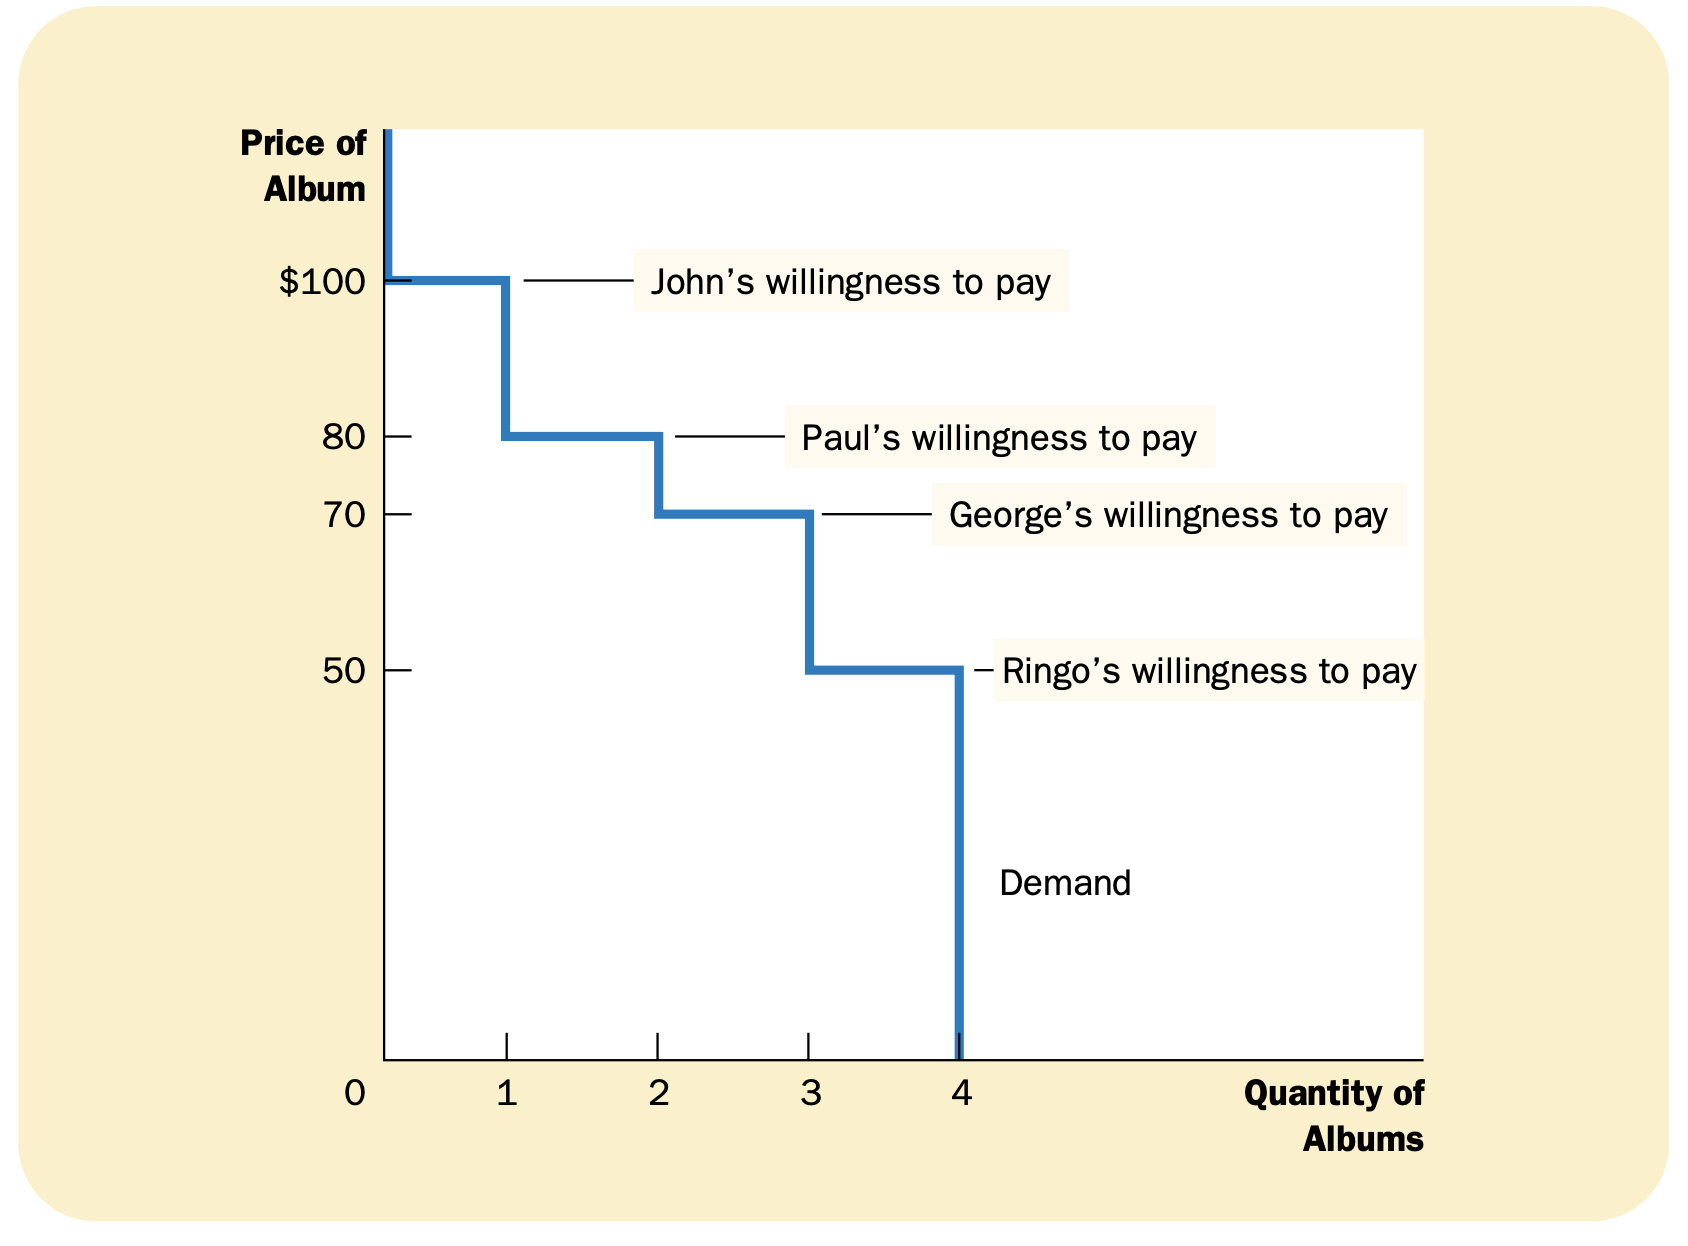
\includegraphics[width=\textwidth]{pics/willingness-to-pay}
  \caption{支付意愿}
  \label{fig:willingness-to-pay}
\end{figure}

\begin{figure}[!ht]
  \centering
  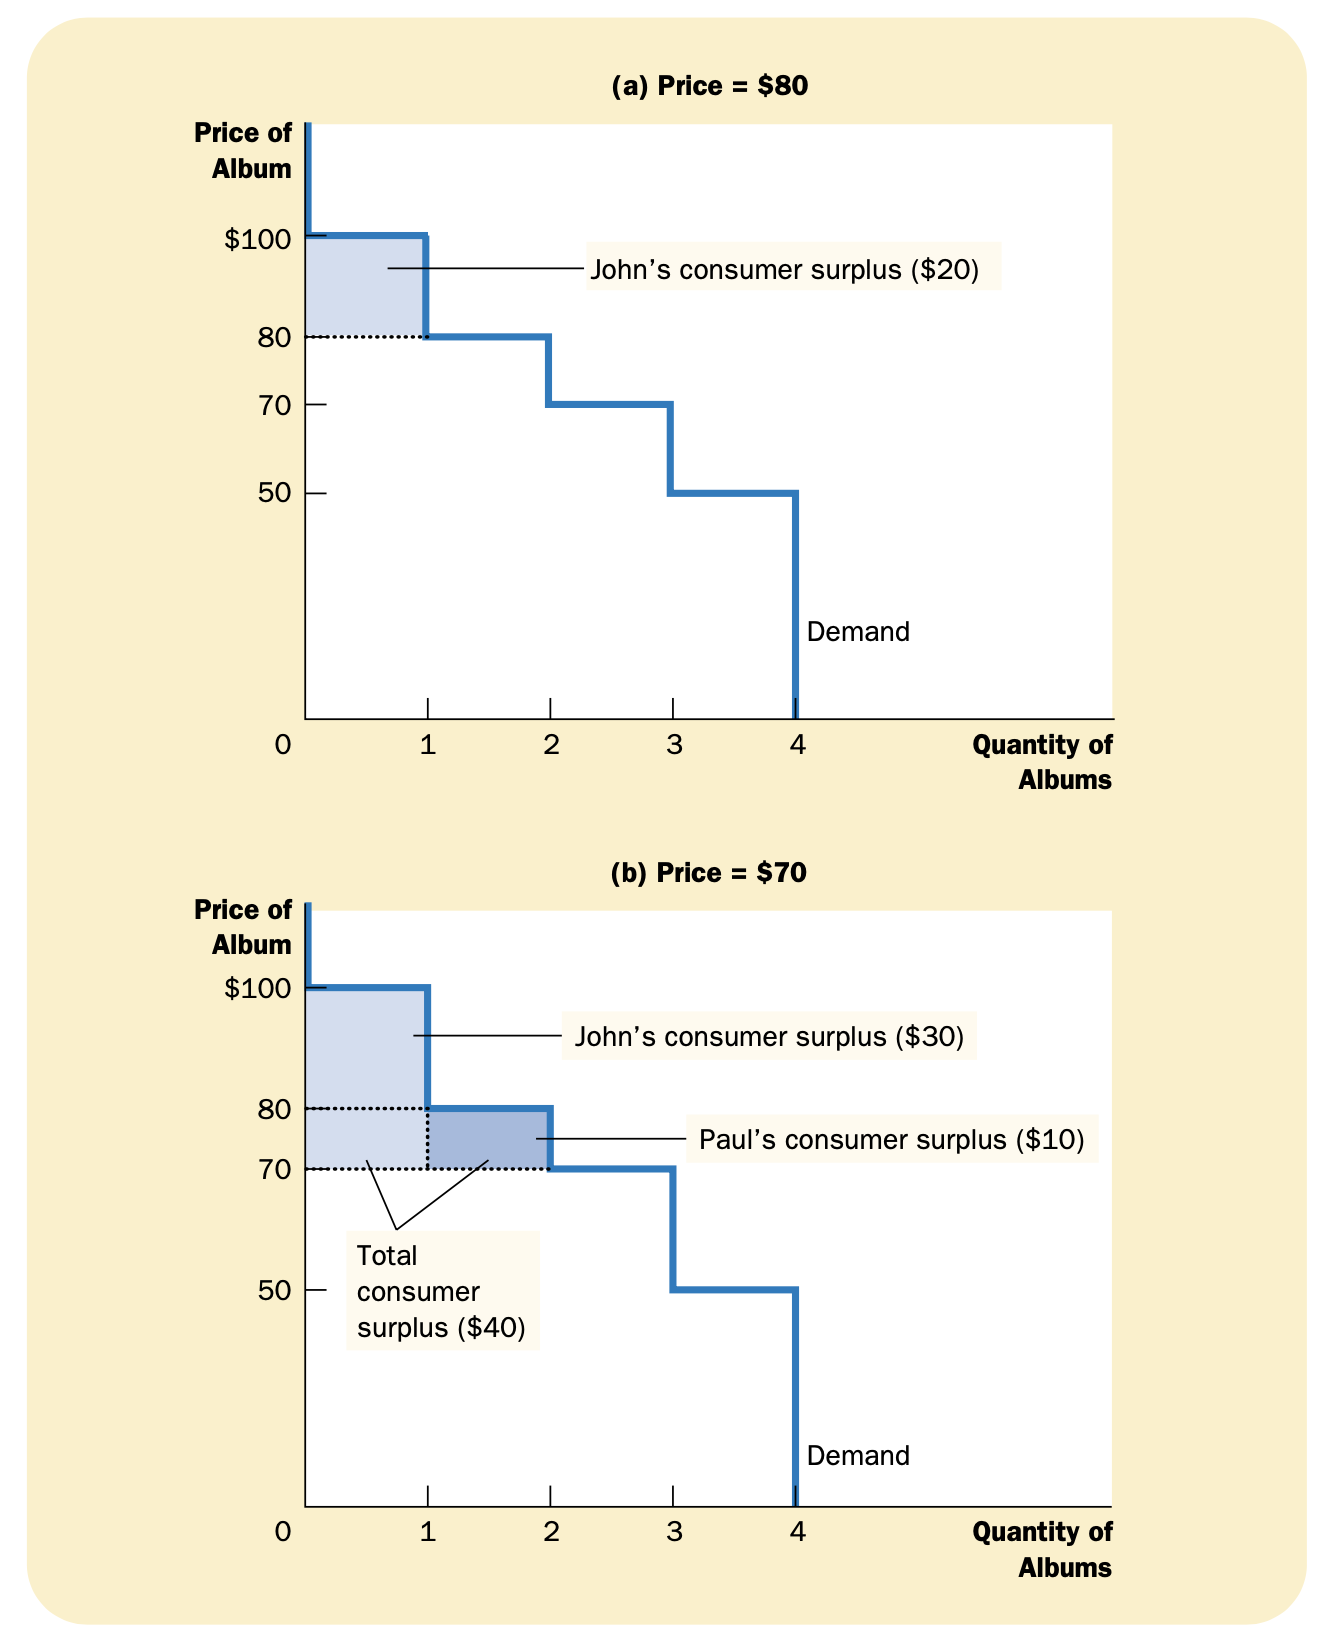
\includegraphics[width=\textwidth]{pics/consumer-surplus}
  \caption{消费者剩余}
  \label{fig:consumer-surplus}
\end{figure}

图\ref{fig:willingness-to-pay}和\ref{fig:consumer-surplus}表明:
需求曲线以下和价格以上的面积衡量一个市场上的消费者剩余。


\subsection{价格降低如何增加消费者剩余}

\begin{figure}[H]
  \centering
  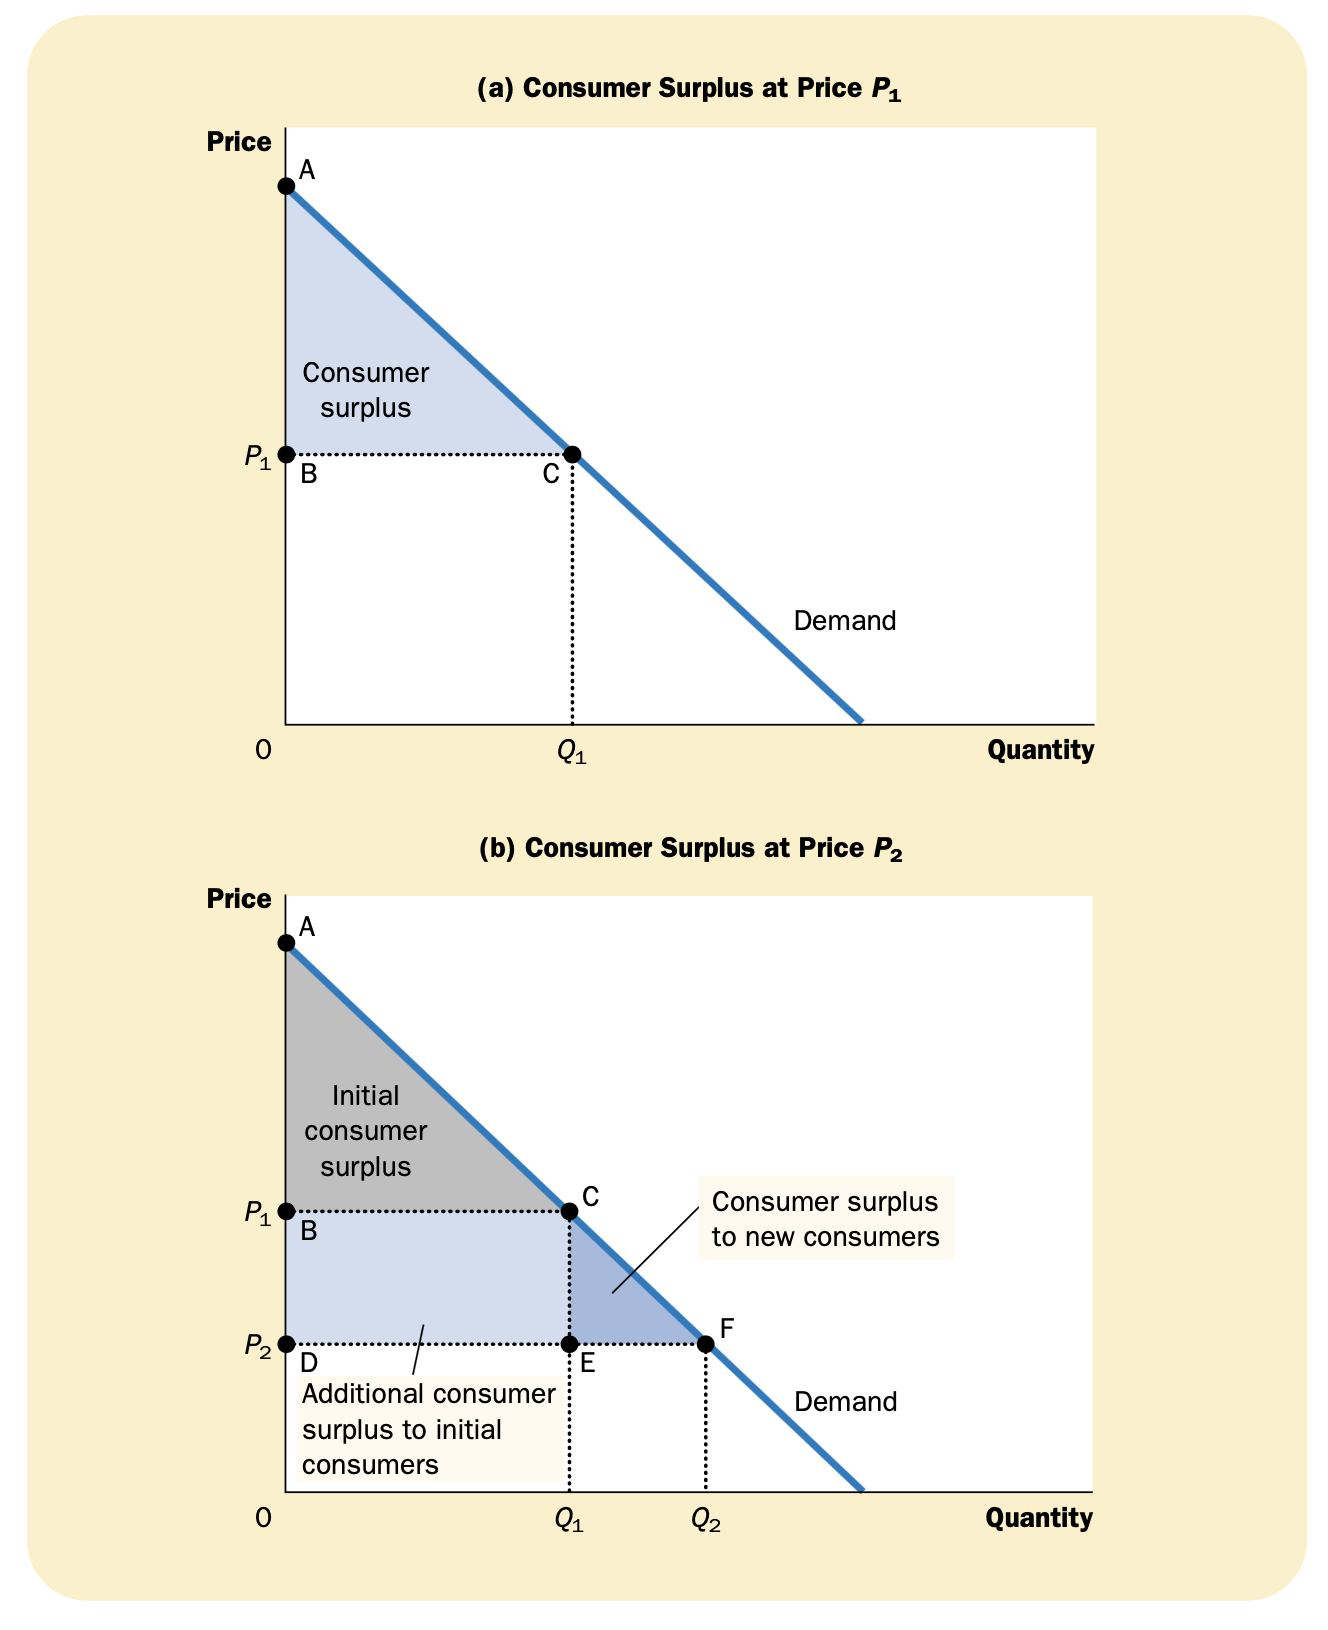
\includegraphics[width=\textwidth]{pics/consumer-surplus2}
  \caption{价格如何影响消费者剩余}
  \label{fig:consumer-surplus2}
\end{figure}


消费者剩余某种程度上不失为经济福利的一种好的衡量标准。

\section{生产者剩余}

\subsection{成本与销售意愿}

成本衡量卖者愿意出售其服务的意愿。

生产者剩余(producer surplus)是卖者得到的量减去其生产成本。
生产者剩余衡量卖者从参与市场中得到的利益。


\subsection{用供给曲线衡量生产者剩余}

边际卖者是如果价格再降低一点就首先离开市场的卖者。


\begin{figure}[!ht]
  \centering
  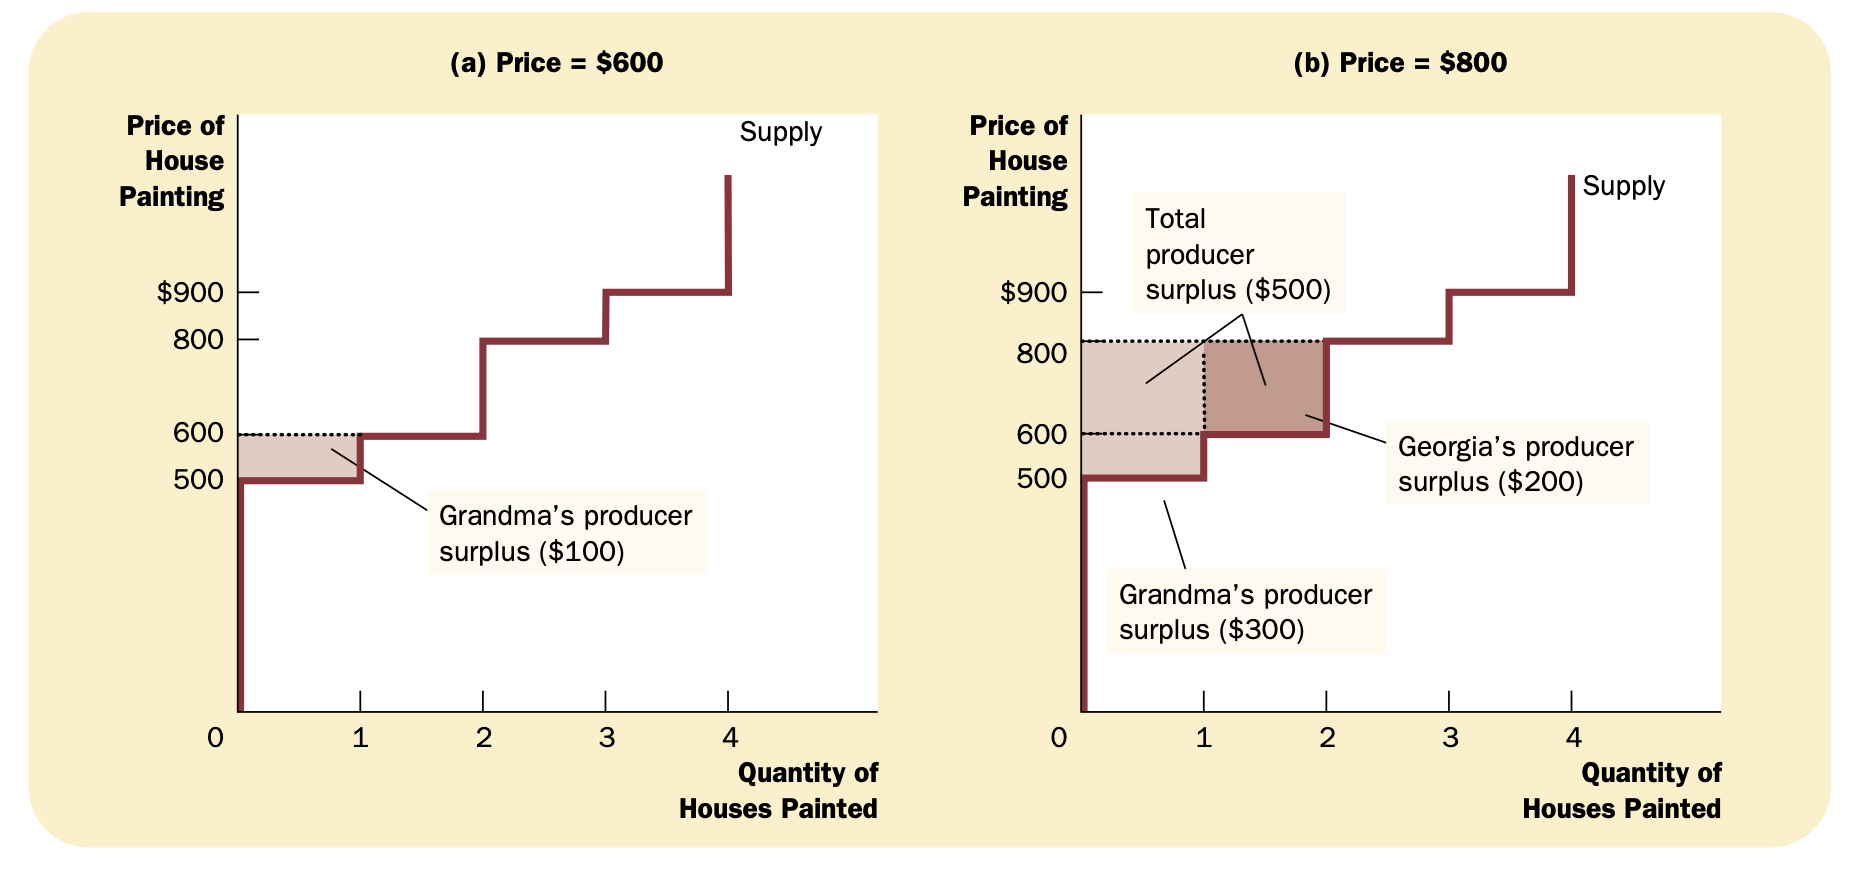
\includegraphics[width=\textwidth]{pics/producer-surplus}
  \caption{生产者剩余}
  \label{fig:producer-surplus}
\end{figure}

图\ref{fig:producer-surplus}表明:
价格之下和供给曲线以上的面积衡量一个市场上的生产者剩余。


\subsection{价格上升如何增加生产者剩余}

\begin{figure}[H]
  \centering
  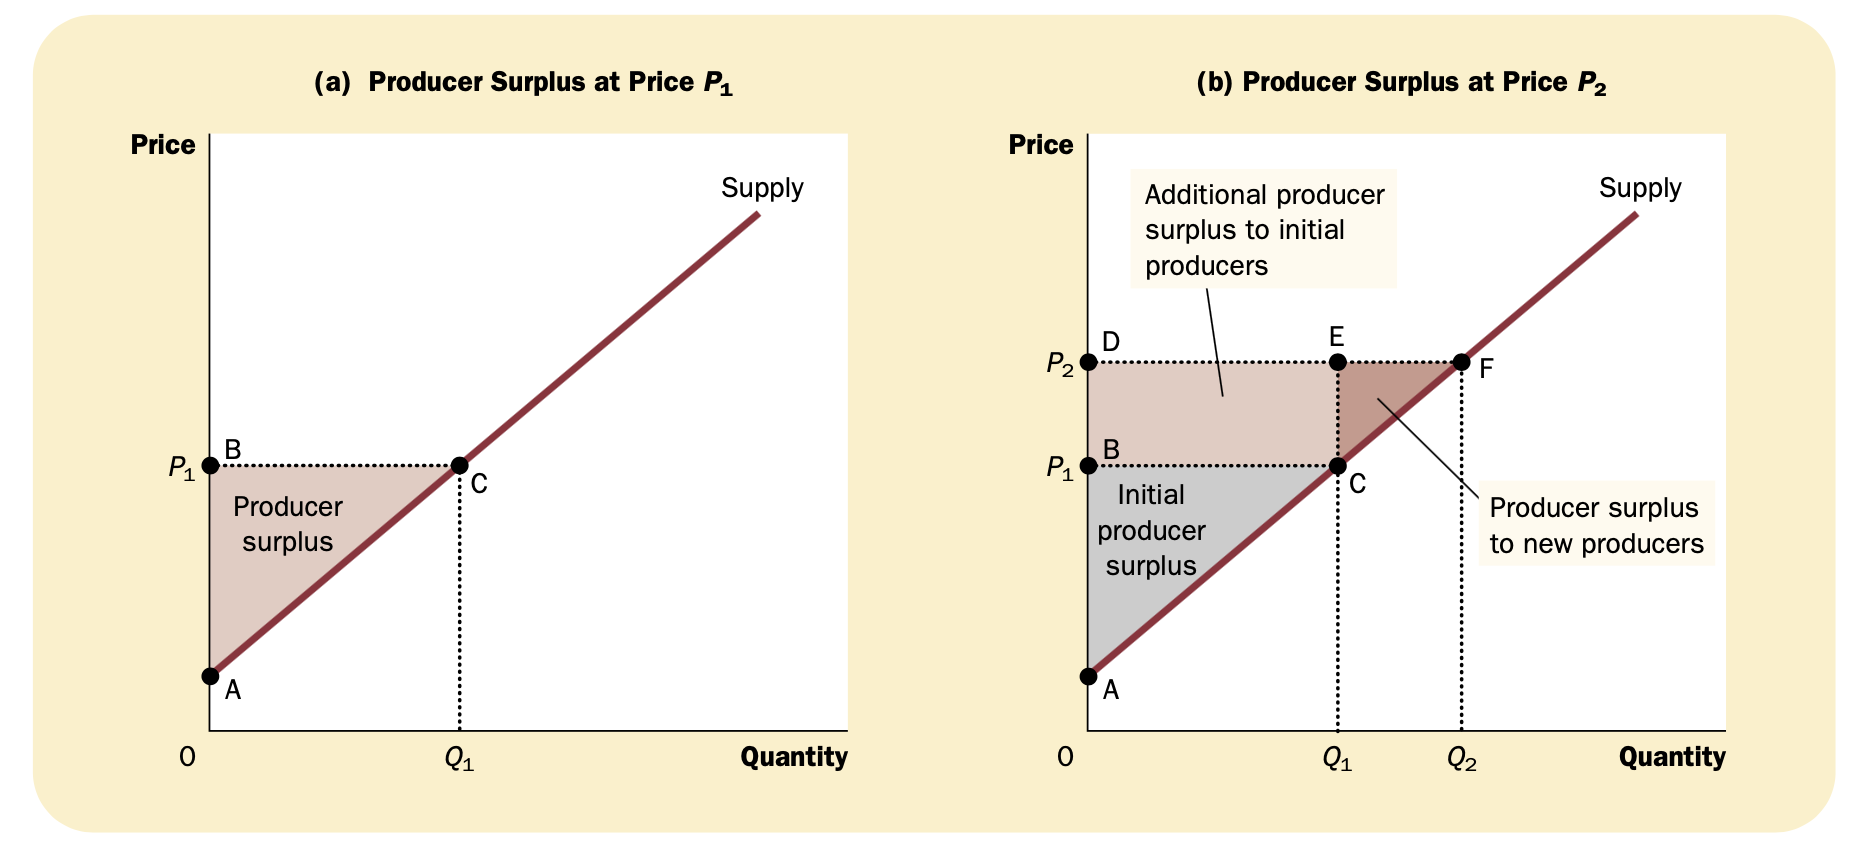
\includegraphics[width=\textwidth]{pics/producer-surplus2}
  \caption{价格上升如何增加生产者剩余}
  \label{fig:producer-surplus2}
\end{figure}


生产者剩余量某种程度上可以用来衡量卖者的福利。


\section{市场效率}



如何衡量社会的经济福利?
一种可能的衡量指标是消费者剩余与生产者剩余的总和,
我们称之为总剩余。


\begin{equation}
  \text{消费者剩余} = \text{买者的评价} - \text{买者支付的量}
\end{equation}
\begin{equation}
  \text{生产者剩余} = \text{卖者得到的量} - \text{卖者的成本}
\end{equation}

因为:
\begin{equation}
  \text{买者支付的量} = text{卖者得到的量}
\end{equation}

所以:
\begin{equation}
  \text{总剩余} = \text{买者的评价} - \text{卖者的成本}
\end{equation}


如果资源配置使总剩余量最大化,
我们可以说,
这种配置是\keyword{有效率}的。
如果一种配置是无效率的,
那么,买者和卖者之间交易的一些潜在的利益就还没有实现。
例如,如果一种物品不是由成本最低的卖者生产的,
配置就是无效率的,
在这种情况下,
将生产从高成本生产者转给低成本生产者就会降低卖者的总成本并增加总剩余。
同样,
如果一种物品不是对这种评价最高的买者消费,
配置也是无效率的。
在这种情况下,将物品的消费从评价低的买者转给评价高的买者就会增加总剩余量。


平等:市场上的各个买者与卖者是否有相似的经济福利水平。


在本质上,
从市场贸易中获得的利益就像一块要在市场参与者间分配蛋糕。
效率问题涉及的蛋糕是否尽可能地做大。
平等问题涉及的是如何把蛋糕切成小块,
以及如何在社会成员中进行分配。




\begin{figure}[!ht]
  \centering
  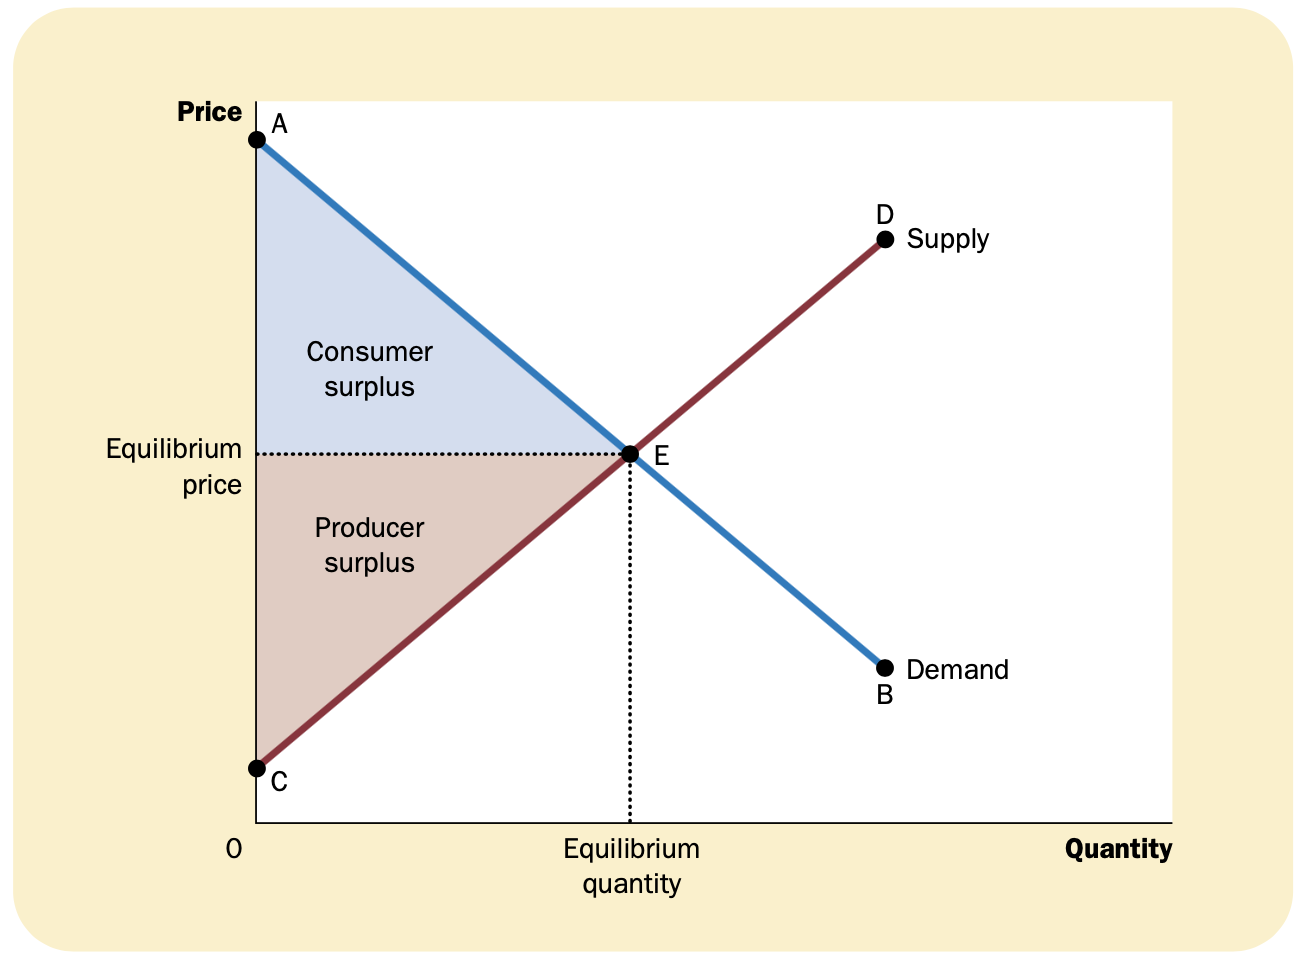
\includegraphics{pics/market-equilibrium}
  \caption{市场均衡时的消费者剩余与生产者剩余}
  \label{fig:market-equilibrium}
\end{figure}

\begin{figure}[!ht]
  \centering
  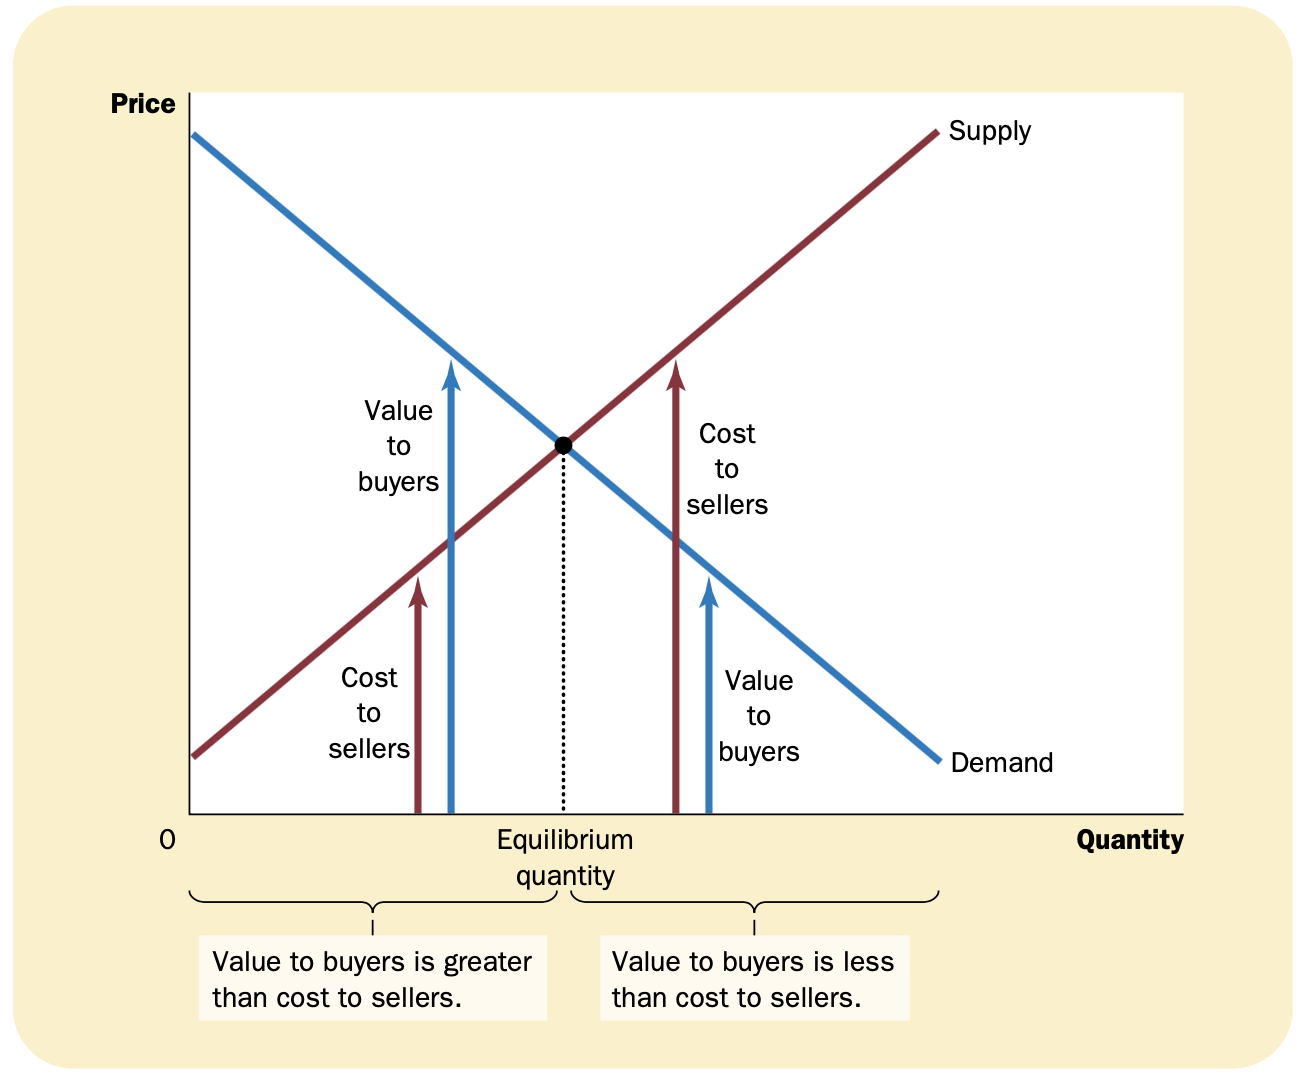
\includegraphics{pics/market-equilibrium2}
  \caption{均衡数量的效率}
  \label{fig:market-equilibrium2}
\end{figure}


从图\ref{fig:market-equilibrium}和\ref{fig:market-equilibrium2}可得出如下结论:
\begin{itemize}
\item 自由市场把物品的供给分配给对这些物品评价高的买者,这种评价用买者的支付意愿来衡量。
\item 自由市场将物品的需求分配给能够以最低成本生产这些物品的卖者。
\item 自由市场生产出使消费者剩余和生产者剩余的总和最大化的物品量。
\end{itemize}


\section{结论}

为了得出市场有效率的结论,
我们做出了一些关于市场如何运行的假设。
当这些假设不成立时,
关于市场均衡有效率的结论可能就不再正确了。


这些假设中有两个最重要的假设:
\begin{itemize}
\item 市场时完全竞争的。
\item 市场结果只影响参与市场的买者和卖者。
\end{itemize}


在现实世界中,在一些市场上,某个单个买者或者卖者(或一小群买者或卖者)可以控制市场价格。
这种影响价格的能力被称为\keyword{市场势力}。

在现实世界中,买者和卖者的决策有时会影响那些根本不参与市场的人。
污染是市场结果影响市场参与者以外的人的一个典型例子。
市场的这种副作用被称为\keyword{外部性}。

市场势力和外部性是一种被称为\keyword{市场失灵}的普遍现象的例子,
市场失灵是指一些不受管制的市场不能有效地配置资源。
当出现市场失灵时,公共政策有可能纠正这些问题并提高经济效率。
